\begin{question}
\noindent The diagram shows a circle with centre $O$. $AB$ is a diameter of the circle, and $C$ is a point on the circumference.

\begin{center}
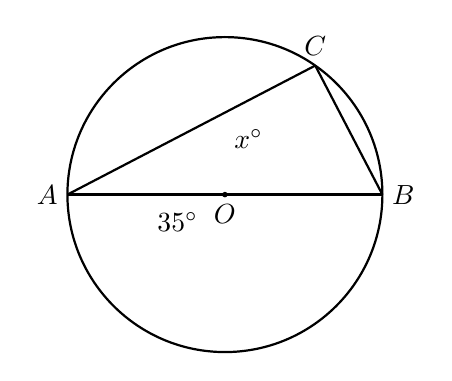
\begin{tikzpicture}[scale=2]
    \coordinate (O) at (0,0);
    \coordinate (A) at (180:1);
    \coordinate (B) at (0:1);
    \coordinate (C) at (55:1);

    \draw[thick] (0,0) circle (1);
    \fill[black] (O) circle (0.5pt);
    \node[below] at (O) {$O$};

    \draw[thick] (A) -- (B);
    \draw[thick] (A) -- (C);
    \draw[thick] (C) -- (B);

    \node[left] at (A) {$A$};
    \node[right] at (B) {$B$};
    \node[above] at (C) {$C$};

    \node at (0.15,0.35) {$x^\circ$};

    \node[below] at (-0.3,-0.05) {$35^\circ$};
\end{tikzpicture}
\end{center}

\noindent Angle $CAB = 35^\circ$.

\noindent Find the size of angle $x$, marked at $C$.

\vspace{4cm}

\begin{flushright}
    \answerequnit{x}{$^\circ$}{2}
\end{flushright}
\end{question}
